% =====================================================================
% DRAFT — Interpretability for Discovery @ NeurIPS 2026 workshop
% 5 pages main text. References and appendices do NOT count.
% Double-blind: no names, affiliations, acknowledgements, or repo URLs.
%
% TO COMPILE: download the workshop template zip from
%   https://interpretability4discovery.github.io/cfp.html
% put neurips_2026.sty next to this file, then compile on Overleaf.
%
% EVERY NUMBER BELOW IS TAGGED WITH ITS SOURCE IN A % COMMENT.
% Verify each one against runs/ before submitting — repo rule is
% "numbers trace to artifacts", and a writeup is not an artifact.
% =====================================================================
\documentclass{article}
\usepackage{neurips_2026}   % NO [final] — submission mode: anonymous + line numbers

\usepackage[utf8]{inputenc}
\usepackage[T1]{fontenc}
\usepackage{hyperref}
\usepackage{url}
\usepackage{booktabs}
\usepackage{amsmath}
\usepackage{amssymb}
\usepackage{graphicx}
\usepackage{microtype}

\title{Extraction works, the contrast does not:\\
positive controls for difference-in-means directions}

\author{Anonymous authors\\Paper under double-blind review}

\begin{document}
\maketitle

\begin{abstract}
Difference-in-means directions are a standard interpretability tool: run two
contrasting prompt sets, subtract mean activations, and treat the result as a
direction encoding the contrast. We report a case where this procedure returns
directions that are unstable across data splits for most of ten social-bias
categories in five open-weight models --- only two clear the bar, and six clear
it in no model at all, including all three race-related categories --- while the
\emph{same} capture site, estimator, and split-half procedure recovers a control
contrast at split-half cosine $0.86$--$0.92$. The positive control is what licenses the negative: the
pipeline is not broken, the contrast is not linearly present at the site we
probe. We further exhibit a configuration that passes the two controls
a steering result is normally asked for---a $7.0\times$ margin over a
norm-matched random direction, and a clean sign-flip response---and show that
two cheap non-standard checks dissolve it: the category's own direction beats an
unrelated category's by only $1.28\times$, while the choice of \emph{which items
are steered} changes the effect by $4.4\times$, and the sign-flip control fails
once the dose is raised. We also report a forking path we caught in our own
analysis, where a regularisation choice made for a stated reason unrelated to
the outcome moves a clustering result from $p=0.179$ to $p=0.030$. We report what
predicts extractability---activation-space separation, not behavioural
bias---and catalogue silent failure modes from an audit of our earlier pipeline,
including an indexing bug that reduced a steering vector to a scalar offset while
still producing a plausible headline effect.
\end{abstract}

% =====================================================================
\section{Introduction}
% =====================================================================

Interpretability increasingly aims to produce knowledge that transfers out of
the model and into a domain. That ambition puts weight on a question that is
easy to skip: when a fitted direction fails to behave as expected, was the
concept absent, or was the instrument broken? The two are routinely confounded,
and the failure is usually resolved in favour of whichever answer the paper
needs.

We take a case where the answer can be separated. Working from BBQ
\citep{parrish2022bbq} social-bias categories across five open-weight models, we
fit difference-in-means directions for a per-category bias margin, and evaluate
them by split-half stability: extract from two random halves of the data, and
ask whether the two directions agree.

Our contributions are:

\begin{enumerate}
\item \textbf{Two pre-specified positive controls} --- fixed in code and
committed before the runs they gate, though not pre-registered in the formal
sense --- that separate instrument failure from construct absence: a behavioural
control establishing the scorer is valid, and an extraction control establishing
the pipeline recovers a direction it should recover, at matched $n$ through an
identical code path.
\item \textbf{A negative result licensed by those controls.} Bias-margin
directions reproduce at split-half cosine $-0.45$ to $+0.82$; only two of ten
categories clear the floor in every model that produced any, and every
race-related category fails in every model.
\item \textbf{Evidence that standard steering controls are insufficient.} We
exhibit a cell passing both the random-control and sign-flip checks, and show
that a cross-category control and a dose sweep---neither standard, both
cheap---remove the interpretation.
\item \textbf{A forking path, reported rather than resolved.} The same
clustering question yields $p=0.179$ under our default estimator and $p=0.030$
under a regularised one, with the regularisation chosen for a reason unrelated
to the outcome. We report both.
\item \textbf{A catalogue of silent failure modes} recovered by auditing our own
prior pipeline, each of which produced plausible results while being wrong.
\end{enumerate}

We report only what the design supports. Where a result rests on a tuned
hyperparameter or a small $n$, we say so in the same sentence as the number.

% =====================================================================
\section{Setup}
% =====================================================================

\paragraph{Models.} Five open-weight instruction-tuned models spanning three
families and 1.8B--14B parameters: \texttt{Qwen/Qwen1.5-1.8B-Chat}
($d_{\mathrm{model}}{=}2048$), \texttt{google/gemma-2b-it} ($2048$),
\texttt{01-ai/Yi-6B-Chat} ($4096$), \texttt{Qwen/Qwen1.5-7B-Chat} ($4096$) and
\texttt{Qwen/Qwen1.5-14B-Chat} ($5120$).
% SOURCE: hf_id and d_model read from runs/full_{qwen18,gemma2b,yi6b,qwen7b,
% qwen14b}/report.json. ACTION: add immutable revision SHAs if the manifests
% carry them; a bare model name is not reproducible provenance.

\paragraph{Directions.} For each BBQ category we form a per-item bias margin
over $n{=}600$ items ($n{=}432$ for Sexual\_orientation, $598$ for
Gender\_identity) and extract a difference-in-means direction from the residual
stream at the final prompt token. Directions are unit-normalised.

\paragraph{Reproducibility criterion.} We split the data into random halves,
extract independently from each, and record the cosine between the two
directions. Over 10 such splits we report the $q_{05}$ as the \emph{floor}. A
direction is \emph{reproducible} if its floor clears $0.500$. For calibration,
two \emph{random} directions in these spaces agree at cosine $0.014$--$0.022$,
so the $0.500$ bar sits far above chance and the quantity being thresholded is
not noise-dominated.

We state the provenance of that constant plainly, because it is a limitation and
not a design feature. It was \textbf{not} pre-registered: it was fixed after an
initial run returned floors of $-0.202$ to $0.423$, and calibrated against the
extraction control below, which reproduces at $q_{05}=0.88$ on the same model
through the same code path, so a working direction clears it with room to spare.
Because the constant is post-hoc we report its sensitivity rather than defend its
value. The qualitative conclusion is unchanged for any threshold in
$[0.30,0.80]$: Disability\_status clears in at least two models throughout that
range, and every race-related category fails at every value of it --- the maximum
floor over all $15$ race model-category pairs is $+0.218$, below even a $0.30$
bar.
% SOURCE: random_floor fields — 0.0221 (qwen-1.8b, _extraction_positive_control.json),
% 0.0140 (qwen-14b), 0.0156 (qwen-7b).

\paragraph{Two estimators.} We report both a plain difference-in-means over
extreme-margin quintiles (the \emph{default} estimator) and a ridge-regularised
probe (the \emph{tuned} estimator, $\alpha{=}10^{6}$). This distinction is
load-bearing and we keep it explicit throughout: the two estimators give
different floors and, as Section~\ref{sec:structure} shows, different answers.

\paragraph{Scoring.} Option likelihoods are scored with no option list in the
prompt, so the measurement does not depend on the model following a
multiple-choice format.

% =====================================================================
\section{Two positive controls}
% =====================================================================

\subsection{The scorer is valid}

On \emph{disambiguated} BBQ items the context identifies the correct referent,
so there is a right answer and accuracy is meaningful. The gate---accuracy
$\geq 50\%$ and $z \geq 3$, committed before the runs reported here---passes for 8 of 10
categories (Table~\ref{tab:posctrl}).
% SOURCE: results/writeups/08-results-2026-08-20.md §1, qwen-1.8b.

\begin{table}[h]
\centering
\caption{Behavioural positive control on disambiguated items, \texttt{qwen-1.8b}.
Chance is $1/3$. Two categories fail the pre-fixed gate and are dropped.}
\label{tab:posctrl}
\begin{tabular}{lrr}
\toprule
category & accuracy & $z$ \\
\midrule
Religion             & 64.0\% & $+8.0$ \\
Race\_x\_SES         & 62.0\% & $+7.4$ \\
Race\_ethnicity      & 61.3\% & $+7.3$ \\
Race\_x\_gender      & 60.7\% & $+7.1$ \\
Gender\_identity     & 58.7\% & $+6.6$ \\
Nationality          & 56.0\% & $+5.9$ \\
Age                  & 55.3\% & $+5.7$ \\
Sexual\_orientation  & 55.3\% & $+5.7$ \\
\midrule
Physical\_appearance & 49.3\% & $+4.2$ \quad(dropped) \\
Disability\_status   & 44.7\% & $+2.9$ \quad(dropped) \\
\bottomrule
\end{tabular}
\end{table}

Dropping these two matters, and the pattern is worth stating carefully. In
\texttt{qwen-1.8b} the gate removes Physical\_appearance and
Disability\_status; the same gate passes all ten categories in
\texttt{qwen-7b} and \texttt{qwen-14b}, where those two reach $65.3\%$/$59.3\%$
and $68.7\%$/$67.3\%$ accuracy respectively.
% SOURCE: positive_control blocks in runs/probe_tuned_qwen7b_a1e6/report.json
% and runs/probe_tuned_qwen14b/report.json, n=150 per category.
The exclusion is therefore a property of the smallest model, not of the
categories.

That interacts with everything below: the two categories \texttt{qwen-1.8b}
cannot comprehend are precisely the two whose directions extract most reliably
in every larger model. Comprehension appears to gate extractability, which is
also why \texttt{qwen-1.8b} yields no reproducible direction at all. Separately,
Physical\_appearance was the only category showing stereotype preference under an
earlier generation-based method ($z=+3.1$) --- a bias signal from a category the
model cannot resolve even when told the answer, which the gate removes before it
can become a finding.

\subsection{The extraction machinery works}

We extract a direction for \emph{topic identity} --- which subject a question is
about --- through the identical capture site, estimator, and split-half
procedure, at matched $n{=}320$. Three such contrasts on \texttt{qwen-1.8b}
(Race\_ethnicity vs.\ Gender\_identity, Religion vs.\ Age, and Nationality vs.\
Sexual\_orientation) give floors of $q_{05}=0.882$, $0.893$ and $0.871$, with
medians $0.899$, $0.912$ and $0.906$. The control was also run on
\texttt{gemma-2b} and \texttt{yi-6b}; see Appendix.
% SOURCE: runs/_extraction_positive_control.json — all six values verified
% exactly against the artifact, n=320, 10 splits, random_floor 0.0221.

The residual stream at the final prompt token cleanly encodes what a question is
about, and our pipeline recovers it. This is the load-bearing control: any
subsequent failure of the bias contrast cannot be attributed to the capture
site, the estimator, or the split-half procedure, because all three are shared.

% =====================================================================
\section{The bias contrast does not reproduce}
% =====================================================================

Against a control reproducing at $0.86$--$0.92$, bias-margin directions span
$-0.45$ to $+0.82$ (Table~\ref{tab:floors}).
% SOURCE: results/writeups/10-EXPERIMENT-1-FINDINGS.md §3 floor table.

\begin{table}[h]
\centering
\caption{Split-half floor ($q_{05}$) per category and model, \textbf{default
estimator}. Bold clears the pre-fixed $0.500$ bar. Dashes are categories that
did not run for that model. Random directions in these spaces agree at
$0.014$--$0.022$.}
\label{tab:floors}
\begin{tabular}{lrrrrr}
\toprule
category & qwen-7b & yi-6b & gemma-2b & qwen-14b & qwen-1.8b \\
\midrule
Disability\_status   & \textbf{0.700} & \textbf{0.605} & \textbf{0.818} & \textbf{0.820} & --- \\
Physical\_appearance & \textbf{0.785} & \textbf{0.614} & \textbf{0.511} & \textbf{0.648} & --- \\
Religion             & 0.316 & $-0.454$ & $-0.163$ & \textbf{0.686} & $-0.008$ \\
Age                  & 0.194 & 0.177 & 0.161 & \textbf{0.754} & 0.423 \\
Race\_x\_gender      & 0.218 & 0.204 & $-0.044$ & 0.072 & 0.138 \\
Nationality          & $-0.020$ & 0.296 & $-0.038$ & 0.279 & 0.057 \\
Sexual\_orientation  & $-0.104$ & $-0.304$ & 0.056 & 0.161 & $-0.202$ \\
Race\_x\_SES         & $-0.150$ & 0.089 & $-0.165$ & $-0.105$ & 0.017 \\
Race\_ethnicity      & $-0.214$ & $-0.230$ & $-0.013$ & $-0.204$ & $-0.115$ \\
Gender\_identity     & $-0.177$ & --- & --- & 0.081 & $-0.072$ \\
\bottomrule
\end{tabular}
\end{table}

\begin{figure}[t]
\centering
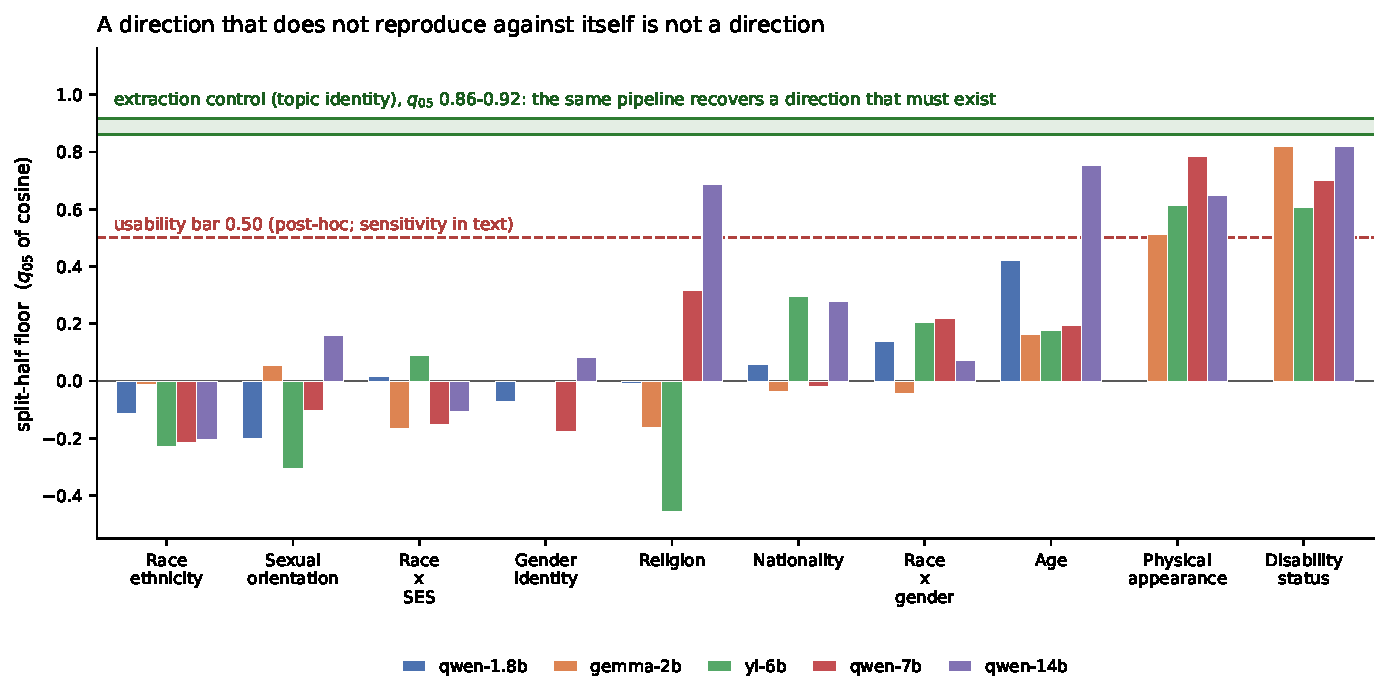
\includegraphics[width=\linewidth]{figures/floors.pdf}
\caption{Split-half extraction floor ($q_{05}$ of the cosine between directions
fit on disjoint halves) for every category and model. Categories are ordered by
mean floor. The green band is the extraction control --- a topic-identity
direction pushed through the identical capture site, estimator and split
procedure at matched $n$ --- which reproduces at $q_{05}=0.86$--$0.92$ across
three models. The control is what makes the rest of the plot readable: the
pipeline demonstrably recovers a direction that exists, so the bias contrast's
failure is a property of the contrast. Every race-related category sits at or
below zero in every model, and a floor reliably below zero means the two halves
recover systematically opposed directions --- what fitting noise under a sign
convention looks like, not a weak positive.}
\label{fig:floors}
\end{figure}

Two observations survive across models. Disability\_status and
Physical\_appearance produce a reproducible direction in every model that
produced any; three models agree exactly on that pair and nothing else
(Jaccard $1.00$). And every race-related category---Race\_ethnicity,
Race\_x\_gender, Race\_x\_SES---fails in every model.

Negative split-half cosines deserve comment. A cosine near $0$ is what two
random directions give; a cosine reliably \emph{below} zero means the two halves
recover systematically opposed directions, which is what fitting noise with a
sign convention looks like. It is not a weaker version of a positive result.

\paragraph{What predicts extractability.} The strongest predictor of a
category's floor is the norm of its direction --- how separated the two groups
are in activation space --- not how biased the model behaves on it. Across the
five models, floor correlates with direction norm at $+0.77$, $+0.81$, $+0.90$,
$+0.91$ and $+0.95$ (Pearson, $n{=}8$--$10$ categories per model), against
$+0.66$ to $+0.77$ for the model's behavioural tilt. Effect size, the mean
margin divided by its standard deviation, sits between the two at $+0.84$ on
\texttt{qwen-14b}: a category yields a direction when the model leans the same
way \emph{consistently} across its items, not merely when it leans hard.
% SOURCE: recomputed 2026-08-29 from runs/full_*/direction_norms.json
% (frobenius_norm vs floor): qwen-1.8b +0.808, gemma-2b +0.945, yi-6b +0.765,
% qwen-7b +0.904, qwen-14b +0.912. Behavioural tilt from
% runs/_cross_model_final.json (mean_margin vs floor): +0.689/+0.660/+0.689/
% +0.769/+0.726. Effect size +0.835 from runs/full_qwen14b/heterogeneity.json.
% All four previously published norm figures reproduce to three decimals;
% qwen-7b is new (its norms artifact was the only one missing).

We also tested and refuted the natural explanation that heterogeneous categories
fail because they bundle unrelated stereotypes: floor against number of distinct
stereotype sets gives $r=-0.079$, and against entropy $r=-0.020$. Religion has
the most heterogeneous stereotype sets of any category and reproduces in one
model; Race\_ethnicity has as many and reproduces nowhere.

\paragraph{A confound this creates, and how it is controlled.} Because a
mean-difference vector's norm scales with the separation between its poles, the
categories that reproduce are exactly the ones with the largest raw directions.
An intervention that adds the unnormalised direction with a fixed coefficient
therefore delivers a \emph{larger dose} to precisely the categories that
reproduce, and any apparent specificity would be confounded with dose. Every
intervention reported in Section~\ref{sec:transfer} uses unit-normalised
directions with the dose carried in the coefficient, so this confound does not
apply to those numbers. We flag it because the norm--floor correlation is strong
enough ($+0.77$ to $+0.95$) that an unnormalised transfer experiment on this data
would be uninterpretable, and that is not obvious from the experiment
description alone.

% =====================================================================
\section{Reproducible directions do not steer selectively}
\label{sec:transfer}
% =====================================================================

A direction that is stable across splits has passed a real test, but stability
is not intervention validity. Restricting to reproducible directions and
sweeping the intervention coefficient:

\begin{table}[h]
\centering
\caption{Mean margin shift under intervention, unit-normalised directions,
restricted to reproducible directions. \emph{own} steers a category with its own
direction; \emph{cross} steers it with another category's; \emph{random} is
norm-matched. \emph{flips} counts categories whose effect inverts under sign
inversion.}
\label{tab:transfer}
\begin{tabular}{llrrrr}
\toprule
model & coeff & own & cross & random & flips \\
\midrule
gemma-2b & 2  & $-0.081$ & $-0.063$ & $+0.011$ & 2/2 \\
gemma-2b & 5  & $-0.221$ & $-0.171$ & $+0.031$ & 1/2 \\
gemma-2b & 10 & $-0.433$ & $-0.361$ & $+0.065$ & 0/2 \\
\midrule
qwen-14b & 2  & $+0.000$ & $+0.004$ & $+0.004$ & 3/4 \\
qwen-14b & 4  & $+0.002$ & $+0.009$ & $+0.007$ & 3/4 \\
qwen-14b & 8  & $+0.004$ & $+0.019$ & $+0.013$ & 2/4 \\
qwen-14b & 16 & $+0.007$ & $+0.033$ & $+0.025$ & 1/4 \\
\bottomrule
\end{tabular}
\end{table}
% SOURCE: runs/full_gemma2b/transfer_test_norm_c{2,5,10}.json and
% runs/full_qwen14b/transfer_test_norm_c{2,4,8,16}.json — summary block fields
% mean_own_effect, mean_cross_effect, mean_random_effect, n_sign_flips_good.

On \texttt{qwen-14b} the own-direction effect is \emph{smaller} than the
cross-direction effect at every dose, and smaller than the norm-matched random
control at three of four. The sign-flip control degrades monotonically with dose,
from 3/4 categories to 1/4. Nothing here supports the direction encoding its
category.

\texttt{gemma-2b} is the interesting case, because at $\mathrm{coeff}{=}2$ it
looks like a success. The own-direction effect is $7.0\times$ the random control
and both categories pass the sign-flip control --- the two checks a steering
result is normally asked for. Reported alone, that reads as evidence the fitted
direction encodes the category.

Two cheap additional comparisons dissolve it. First, own exceeds cross by only
$1.28\times$ ($-0.081$ vs $-0.063$), whereas \emph{which items are being steered}
changes the effect by $4.4\times$: Disability items move $\approx -0.117$ and
Physical items $\approx -0.027$, near-identically under either direction. The
effect is largely a property of what is being steered, not of which direction
steers it. Second, the apparent success does not survive dose escalation --- the
sign-flip control that passes 2/2 at $\mathrm{coeff}{=}2$ passes 1/2 at $5$ and
0/2 at $10$, while the effect size grows fivefold.

This is the pattern \citet{joad2026} report for refusal --- geometrically
distinct directions behaving as a single control under intervention --- observed
here in a different model family and a different dataset. The methodological
point we want to stress is narrower and does not depend on that reading: a
cross-category control and a dose sweep are both cheap, neither is standard, and
either one would have prevented the $\mathrm{coeff}{=}2$ cell from being
reported as a positive result.

\paragraph{Not causal.} This arm used a norm-matched rather than
covariance-matched random control, ran no coherence check on generations, and
had no system-prompt baseline. We report it as a constraint on interpretation,
not as a causal claim.

% =====================================================================
\section{A forking path we caught in our own analysis}
\label{sec:structure}
% =====================================================================

Do the directions that survive cluster into groups? The answer depends entirely
on which estimator is used, and we report both because the contrast is more
instructive than either result.

\begin{table}[h]
\centering
\caption{Clustering against a 200-permutation null. The same question, two
estimators, opposite answers.}
\label{tab:fork}
\begin{tabular}{llrrr}
\toprule
estimator & model & \#\,reproducible & cluster strength & $p$ \\
\midrule
default & qwen-1.8b & 0 & --- & 0.229 \\
default & gemma-2b  & 2 & --- & 1.000 \\
default & yi-6b     & 2 & \multicolumn{2}{l}{not clusterable ($<3$)} \\
default & qwen-7b   & 2 & \multicolumn{2}{l}{not clusterable ($<3$)} \\
default & qwen-14b  & 4 & --- & 0.179 \\
\midrule
tuned ($\alpha{=}10^{6}$) & qwen-14b & 5 & 0.0962 & \textbf{0.030} \\
tuned ($\alpha{=}10^{6}$) & qwen-7b  & 3 & 0.3351 & \textbf{0.005} \\
\bottomrule
\end{tabular}
\end{table}

% SOURCE: default rows — verdict/p_value fields in runs/_cross_model_final.json.
% tuned rows — runs/probe_tuned_qwen14b/report.json (p=0.029850746,
% cluster_strength=0.09621271, null median 0.0473 q95 0.0852 n=200) and
% runs/probe_tuned_qwen7b_a1e6/report.json (p=0.004975124,
% cluster_strength=0.33508, null median 0.0573 q95 0.1378 n=200).

Under the default estimator, \textbf{no model shows structure}. Under a ridge
probe at $\alpha{=}10^{6}$, two models do, one of them at $p=0.005$.

The mechanism is not subtle. Regularisation lifts marginal categories over the
$0.500$ floor---qwen-14b goes from four reproducible directions to five, qwen-7b
from two to three---and three is the minimum at which clustering can be computed
at all. The penalty was chosen by inspecting extraction floors on the same data.
It was not chosen against the clustering statistic or the $p$-value, and the
second model was run at the first model's $\alpha$ without re-tuning, which is
the one thing that makes the replication meaningful. But $\alpha{=}10^{6}$ is
also the value that maximises how many categories clear the bar, and more
categories is what makes the test possible. That is a researcher degree of
freedom sitting directly upstream of the $p$-value.

We therefore do not claim bias directions cluster. We claim that a defensible
analysis choice, made for a stated reason unrelated to the outcome, moves this
question from $p=0.179$ to $p=0.030$, and that reporting only the second would
have been indistinguishable from reporting a finding. The qwen-7b replication at
a fixed $\alpha$ is the strongest version of the positive result and we still do
not think it is enough, because the two models share only three reproducible
categories, so whether they agree on the \emph{arrangement} is untestable rather
than refuted (Pearson $-0.095$, Spearman $+0.500$, over three pairs).

What would settle it: fix $\alpha$ by a rule that does not consult this data
(scaled to $d_{\mathrm{model}}$, say), fix the floor threshold, pre-register
both, and only then look at the $p$-value.

% =====================================================================
\section{Silent failure modes}
\label{sec:defects}
% =====================================================================

Auditing our own pipeline recovered six defects, each of which produced
usable-looking output. We describe three here and three in
Appendix~\ref{app:defects}. We report them because each is invisible in results
and detectable only against artifacts --- which is the same problem the rest of
this paper is about, arriving one level down.

\paragraph{An index that silently became a scalar.} Saved steering vectors were
one-dimensional hidden-width tensors. The intervention indexed them as
\texttt{vector[layer]} and added the result to the whole residual width---adding
a scalar offset, not a direction. The affected runs still produced a clean
headline: unsafe responses rising from $1/99$ to $27/99$ under the ``opinion''
vector. The counts are real; the causal label was false.

\paragraph{A parser that failed toward position, invisibly.} An earlier scoring
design generated a response and parsed which option it named, resolving ties by
earliest mention. The rule was adopted for a real reason --- models state a
choice and then explain themselves, naming the other option, and treating that
as ambiguous discarded a third to a half of responses --- and it fixed that
problem. But it has no negation handling and no question-echo stripping. Of
seven realistic phrasings, three parse wrong, and \emph{every} failure resolves
to whichever option is named first: ``It's not the doctor, it's the nurse''
scores as the doctor. The unparsed rate was visible and we reported it; the
\emph{misparsed} rate is invisible, because a wrong label is byte-identical to a
right one in the saved counts. Since the raw response text was not persisted, it
can no longer be measured at any price. A first-mention-biased parser reproduces
the exact signature we had read as evidence of model-side order sensitivity, so
that reading cannot be separated from the parser's own bias using the data we
kept. The general lesson is not about this parser: a labelling rule whose inputs
are discarded turns a fixable bug into a permanent one.

\paragraph{A selectivity rule that fires on one mechanism.} A single-point
ratio rule of the form $\mathrm{SEL} \geq 2$, intended to separate two
mechanisms, fires with probability $2.0\%$ to $61.5\%$ in simulation while the
world is held fixed at one mechanism and only unmeasurable direction-estimate
quality varies. In part of that range it does not merely lose power but
\emph{inverts}: at $\rho_{\mathrm{stance}}{=}0.85$, $\rho_{\mathrm{harm}}{=}0.55$
the population ratio is $0.59$, so the rule reports the opposite of the truth
while the world has not changed at all.
% SOURCE: runs/_sim/sim_lambda_identifiability_reps600.txt, generated
% 2026-08-29 by analysis/sim_lambda_identifiability.py --reps 600.
% The 2.0%-61.5% endpoints are FROM THAT RUN. RESEARCH_CONTRACT.md §5.1 and
% DECISION_LOG.md D-009 publish 1.8%-64%; the difference is Monte Carlo noise at
% 600 reps. Cite the committed run, not the contract. The 0.59 inversion is a
% population quantity and is identical in every run.

% =====================================================================
\section{Limitations}
% =====================================================================

The negative result is specific: it says a per-category bias margin is not
recoverable as a stable linear direction from the residual stream at the final
prompt token, by difference-in-means, at these scales. It does not say bias is
absent from the models, nor that no site or estimator recovers it. Sparse
autoencoders, other layers and token positions, and non-linear probes are all
untested here. The intervention arm is uncontrolled in the three respects named
above. The clustering result carries a tuned hyperparameter and $n=5$ and $n=3$
categories. Scale is limited to 14B, and all models are instruction-tuned.

% =====================================================================
\section*{Responsible use}
% =====================================================================

This work measures social-bias representations and reports mostly that a
particular measurement does not work. The main foreseeable harm is misreading
that as evidence models are unbiased. It is not: the behavioural control shows
these models do exhibit measurable per-category tilt, and our result concerns
whether that tilt is recoverable as a linear direction at one site, not whether
it exists. A second risk is the mirror image---treating unstable directions as
validated bias detectors and deploying them for auditing, which the split-half
floors here argue against directly. The extraction and evaluation code, the split-half protocol and the
per-category floors will be released with the camera-ready version so that both
readings can be checked rather than taken on trust. The BBQ items we use are a
published benchmark of social-bias contrasts; we generate no new content about
real individuals and add no new demographic annotations.

\bibliographystyle{plainnat}
\begin{thebibliography}{9}

\bibitem[Parrish et al.(2022)]{parrish2022bbq}
Parrish, A. et al.
\newblock BBQ: A hand-built bias benchmark for question answering.
\newblock \emph{Findings of ACL}, 2022.

\bibitem[Arditi et al.(2024)]{arditi2024refusal}
Arditi, A. et al.
\newblock Refusal in language models is mediated by a single direction.
\newblock \emph{NeurIPS}, 2024.

\bibitem[Joad et al.(2026)]{joad2026}
Joad, F., Hawasly, M., Boughorbel, S., Durrani, N., and Sencar, H.~T.
\newblock There is more to refusal in large language models than a single direction.
\newblock arXiv:2602.02132, 2026.

\end{thebibliography}

% =====================================================================
\appendix
\section{Full per-category results}
% =====================================================================
% Generated from runs/ by paper/figures/make_appendix_tables.py.
% Regenerate rather than hand-edit:
%   python paper/figures/make_appendix_tables.py > paper/appendix_tables.tex
% Appendices do not count toward the 5-page limit.
% ==== generated by paper/figures/make_appendix_tables.py - do not hand-edit ====

\begin{table}[h]
\centering
\caption{Models. Exact Hugging Face identifiers as recorded in the run manifests. Immutable revision SHAs were not captured at run time; we record that as a reproducibility gap rather than reconstruct them.}
\label{tab:models}
\begin{tabular}{llrr}
\toprule
short name & Hugging Face id & layers & $d_{\mathrm{model}}$ \\
\midrule
\texttt{qwen-1.8b} & \texttt{Qwen/Qwen1.5-1.8B-Chat} & 24 & 2048 \\
\texttt{gemma-2b} & \texttt{google/gemma-2b-it} & 18 & 2048 \\
\texttt{yi-6b} & \texttt{01-ai/Yi-6B-Chat} & 32 & 4096 \\
\texttt{qwen-7b} & \texttt{Qwen/Qwen1.5-7B-Chat} & 32 & 4096 \\
\texttt{qwen-14b} & \texttt{Qwen/Qwen1.5-14B-Chat} & 40 & 5120 \\
\bottomrule
\end{tabular}
\end{table}

\begin{table}[h]
\centering
\caption{Per-category split-half floor, all models. Each cell is $q_{05}$ / median over 10 splits, with the number of items the direction was fit on. Dashes are categories dropped by the behavioural task control for that model.}
\label{tab:floors-full}
\small
\begin{tabular}{lrrrrr}
\toprule
category & \texttt{qwen-1.8b} & \texttt{gemma-2b} & \texttt{yi-6b} & \texttt{qwen-7b} & \texttt{qwen-14b} \\
\midrule
Age & +0.423 / +0.478 \tiny{(320)} & +0.161 / +0.333 \tiny{(240)} & +0.177 / +0.361 \tiny{(240)} & +0.194 / +0.443 \tiny{(240)} & +0.754 / +0.863 \tiny{(240)} \\
Disability\_status & --- & +0.818 / +0.919 \tiny{(240)} & +0.605 / +0.879 \tiny{(240)} & +0.700 / +0.862 \tiny{(240)} & +0.820 / +0.898 \tiny{(240)} \\
Gender\_identity & -0.072 / +0.065 \tiny{(318)} & --- & --- & -0.177 / +0.107 \tiny{(238)} & +0.081 / +0.212 \tiny{(238)} \\
Nationality & +0.057 / +0.359 \tiny{(320)} & -0.038 / +0.228 \tiny{(240)} & +0.296 / +0.569 \tiny{(240)} & -0.020 / +0.441 \tiny{(240)} & +0.279 / +0.493 \tiny{(240)} \\
Physical\_appearance & --- & +0.511 / +0.854 \tiny{(240)} & +0.614 / +0.732 \tiny{(240)} & +0.785 / +0.859 \tiny{(240)} & +0.648 / +0.765 \tiny{(240)} \\
Race\_ethnicity & -0.115 / +0.048 \tiny{(320)} & -0.013 / +0.146 \tiny{(240)} & -0.230 / +0.023 \tiny{(240)} & -0.214 / +0.220 \tiny{(240)} & -0.204 / +0.031 \tiny{(240)} \\
Race\_x\_SES & +0.017 / +0.239 \tiny{(320)} & -0.165 / +0.183 \tiny{(240)} & +0.089 / +0.247 \tiny{(240)} & -0.150 / +0.098 \tiny{(240)} & -0.105 / +0.219 \tiny{(240)} \\
Race\_x\_gender & +0.138 / +0.380 \tiny{(320)} & -0.044 / +0.120 \tiny{(240)} & +0.204 / +0.362 \tiny{(240)} & +0.218 / +0.298 \tiny{(240)} & +0.072 / +0.311 \tiny{(240)} \\
Religion & -0.008 / +0.139 \tiny{(240)} & -0.163 / +0.101 \tiny{(240)} & -0.454 / -0.039 \tiny{(240)} & +0.316 / +0.619 \tiny{(240)} & +0.686 / +0.783 \tiny{(240)} \\
Sexual\_orientation & -0.202 / -0.065 \tiny{(172)} & +0.056 / +0.235 \tiny{(172)} & -0.304 / -0.084 \tiny{(172)} & -0.104 / +0.020 \tiny{(172)} & +0.161 / +0.382 \tiny{(172)} \\
\bottomrule
\end{tabular}
\end{table}

\begin{table}[h]
\centering
\caption{Extraction positive control, all three models it was run on. A topic-identity contrast through the identical capture site, estimator and split-half procedure at matched $n$. It was not run on \texttt{qwen-7b} or \texttt{qwen-14b}, which is a gap: those are the two models carrying the clustering result.}
\label{tab:control-full}
\begin{tabular}{llrrr}
\toprule
model & topic contrast & $n$ & $q_{05}$ & median \\
\midrule
\texttt{gemma-2b} & Race\_ethnicity vs.\ Gender\_identity & 320 & 0.915 & 0.925 \\
\texttt{gemma-2b} & Religion vs.\ Age & 320 & 0.912 & 0.926 \\
\texttt{gemma-2b} & Nationality vs.\ Sexual\_orientation & 320 & 0.860 & 0.888 \\
\texttt{yi-6b} & Race\_ethnicity vs.\ Gender\_identity & 320 & 0.862 & 0.897 \\
\texttt{yi-6b} & Religion vs.\ Age & 320 & 0.864 & 0.882 \\
\texttt{yi-6b} & Nationality vs.\ Sexual\_orientation & 320 & 0.879 & 0.891 \\
\texttt{qwen-1.8b} & Race\_ethnicity vs.\ Gender\_identity & 320 & 0.882 & 0.899 \\
\texttt{qwen-1.8b} & Religion vs.\ Age & 320 & 0.893 & 0.912 \\
\texttt{qwen-1.8b} & Nationality vs.\ Sexual\_orientation & 320 & 0.871 & 0.906 \\
\bottomrule
\end{tabular}
\end{table}

% control q05 range: 0.860-0.915 over 9 splits
% bias floor range : -0.454-+0.820 over 46 cells
% cells clearing 0.50: 10/46


% =====================================================================
\section{Three further silent defects}
\label{app:defects}
% =====================================================================

These complete the audit summarised in Section~\ref{sec:defects}. Each was
recovered from committed artifacts, and none was visible in any reported number.

\paragraph{A vector-to-model mapping off by rotation.} Model order and vector
file order differed, so each of five runs loaded a different model's vector than
its label claimed --- the run labelled with one model carried another model's
saved payload, and so on around the cycle. Recovered by comparing tensor-storage
hashes rather than file hashes, since the serialisation containers differ while
the payloads do not. Nothing in any output distinguishes an affected run from a
correct one.

\paragraph{Columns that read as transitions and record marginals.} A results
table with arrow-named columns (\texttt{Init->Opin}) records per-arm label
marginals, not transitions. The aggregation increments one bucket per arm from
that arm's single judgement, so no before/after pair is ever formed and no
transition is observable in principle. The column name invites exactly the
reading the data cannot support, and a table read that way inverts its own
meaning. Recovering transitions requires the prompt-level logs, which we still
have; the summary CSV alone cannot yield them at any effort.

\paragraph{An unpinned judge.} Automated judgements used an unversioned hosted
model alias. The alias has since moved, so the exact weights that produced those
labels are unrecoverable, and the judged numbers cannot be reproduced --- only
re-generated under a different judge. Pinning a dated snapshot costs nothing at
run time and is the difference between a reproducible measurement and a
historical one.

\end{document}
